
\subsection{Introducción}
El conversor sigma-delta o delta-sigma según la literatura consultada, tuvo su aparición durante los años 60's y 70's. Aunque su nombre pueda sugerir un tipo de tecnología muy compleja la realidad es que no lo es en términos constructivos. Los moduladores sigma-delta nos permiten alcanzar una digitalización de alta resolución (16bits o 24bits) sin la necesidad de utilizar ADC de ese porte. Esto se consigue dado que este diseño permite alcanzar un nivel de ruido de cuantización equivalente a la de un ADC de mayor porte utilizando un ADC más modesto.


\subsection{Arquitectura}

A continuación presentamos la topología implementada:

\begin{figure}[H]
	\centering
	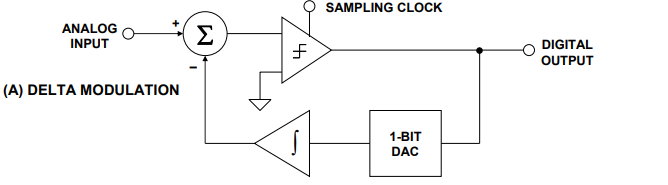
\includegraphics[width=0.7\linewidth]{ImagenesEjercicio2/diagramaEnBloques}
	\caption{Modulador $\Sigma\Delta$ de primer orden}
	\label{fig:diagramaenbloques}
\end{figure}

Como se puede observar el modulador $\Sigma\Delta$ se basa en un circuito con un solo camino de realimentación negativa que incorpora un cuantificador y un DAC en su interior.



\subsection{Modulador}
La salida del modulador $\Sigma\Delta$ es un bit-stream de valores binario arbitrarios. En esta secuencia se encuentra codificada toda la información necesaria para poder reconstruir la señal original. Aún más importante que reconstruir la señal original, es conseguir un valor preciso de la misma en un instante de tiempo. Es decir, poder tomar mediciones. Este tipo de conversores son famosos por la alta resolución que son capaces de proveer. Sin embargo, el limite de su funcionalidad aparece cuando se los quiere utilizar en un ambiente donde la señales cambian de forma abrupta.

\begin{figure}[H]
	\centering
	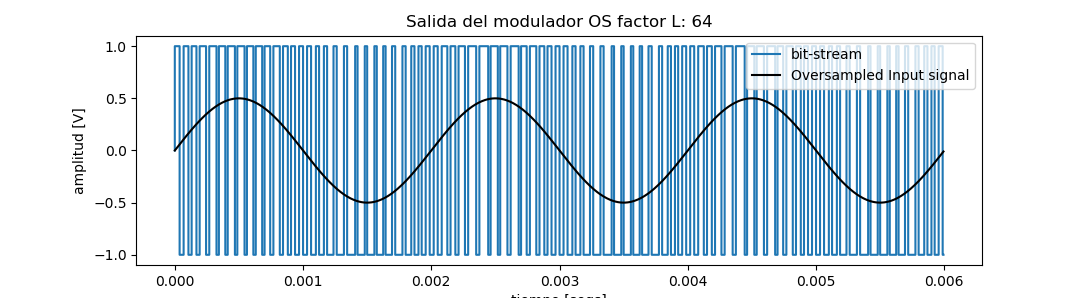
\includegraphics[width=0.7\linewidth]{ImagenesEjercicio2/BitsStream64}
	\caption{}
	\label{fig:bitsstream64}
\end{figure}


\subsection{Noise Shaping}
Una de las más notables características de este tipo de modulación es el efecto llamado \textbf{noise-shaping}. Este efecto provoca que el ruido de cuantización sea "moldeado" hacia las altas frecuencias empujándolo lejos de la banda de interés.


\begin{figure}[H]
	\centering
	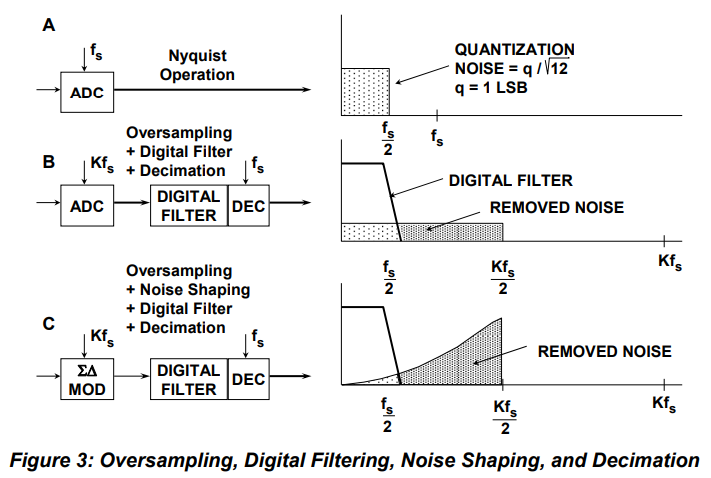
\includegraphics[width=0.7\linewidth]{ImagenesEjercicio2/NoiseShappingAN}
	\caption{}
	\label{fig:noiseshappingan}
\end{figure}


Esto implica que el ruido de cuantización efectivo, dentro de la banda de interés, se ve reducido. Esto es equivalente a pensar que la señal fue cuantizada mediante un cuantizador que tiene un ruido de cuantización proporcional al ruido restante sobre la banda de interés.

A continuación se muestran los resultados obtenidos luego de realizar el periodograma sobre los bits de salida

\begin{figure}[H]
	\centering
	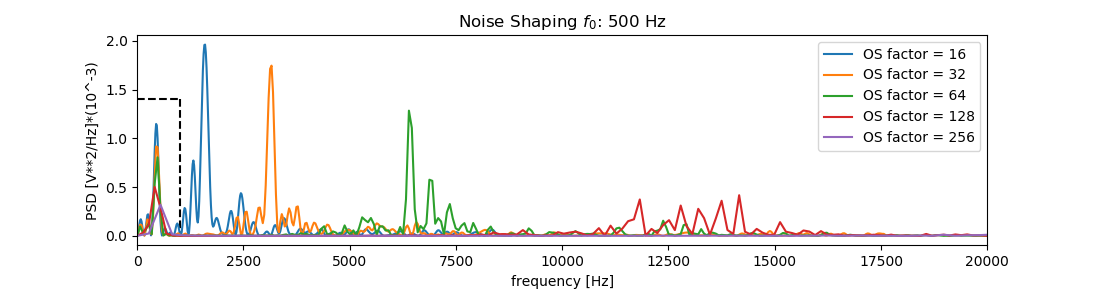
\includegraphics[width=\linewidth]{ImagenesEjercicio2/NoiseShappingDemo1zoom2solid.png}
	\caption{Noise Shapping con diferentes niveles de sobremuestreo}
	\label{fig:noiseshappingdemo1}
\end{figure}
En primer lugar podemos ver que a medida que aumentamos la tasa de oversampling, el ruido de cuantización se aleja más de la banda de interés e incursiona hacia posiciones más elevadas en el espectro.

\begin{figure}[H]
	\centering
	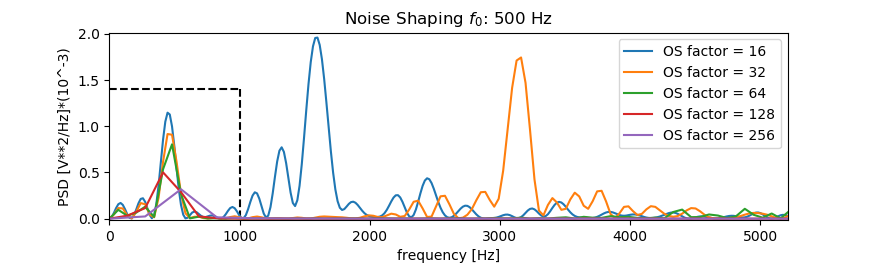
\includegraphics[width=\linewidth]{ImagenesEjercicio2/NoiseShappingSolidZoom.png}
	\caption{Noise Shapping con diferentes niveles de sobremuestreo, acercamiento}
	\label{fig:noiseshappingdemo1}
\end{figure}

Si reescalamos la potencia espectral y la expresamos en dBm conseguimos apreciar notoriamente el noise-shapping.

El pico observado a bajas frecuencias corresponde a la frecuencia fundamental de nuestra información de entrada
\begin{figure}[H]
	\centering
	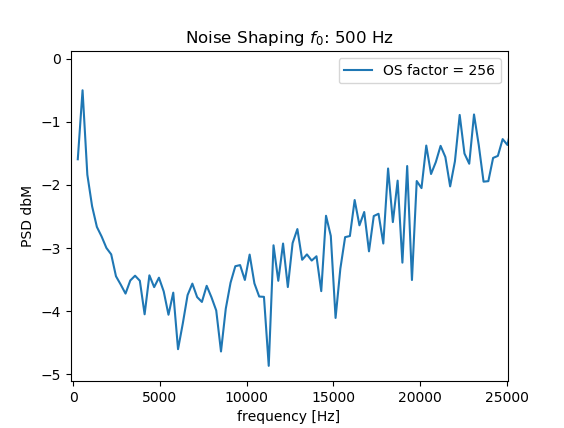
\includegraphics[scale=0.7]{ImagenesEjercicio2/NoiseShappingdbM.png}
	\caption{Noise Shapping}
	\label{fig:noiseshappingdemo1}
\end{figure}
